\chapter{Remaining useful life: Turbofan engines}


\section{Data}

\begin{remark}
    Maintenance can be of three types:
    \begin{descriptionlist}
        \item[Reactive maintenance]
            Repair when something is broken.

        \item[Preventive maintenance]
            Periodically change something, in a conservative way, before it breaks.

        \item[Predictive maintenance]
            Change when something is close to break.
    \end{descriptionlist}

    Remaining useful life (RUL) is a metric useful for predictive maintenance.
\end{remark}

The dataset contains run-to-failure experiments on NASA turbofan engines. Excluding domain specific features, the main columns are:
\begin{descriptionlist}
    \item[\texttt{machine}] Index of the experiment.
    \item[\texttt{cycle}] Time step of the experiment.
    \item[\texttt{rul}] Remaining useful life.
\end{descriptionlist}


From the dataset heatmap, the following can be observed:
\begin{itemize}
    \item Rows with a uniform blue or red color represent features that contain frequent short-lived variations (i.e., peeks) that skew the standard deviation.
    \item Some features show a trend synced with the experiments (see rows around 15 at the y-axis with blue peeks at the end of each experiment).
\end{itemize}
\begin{figure}[H]
    \centering
    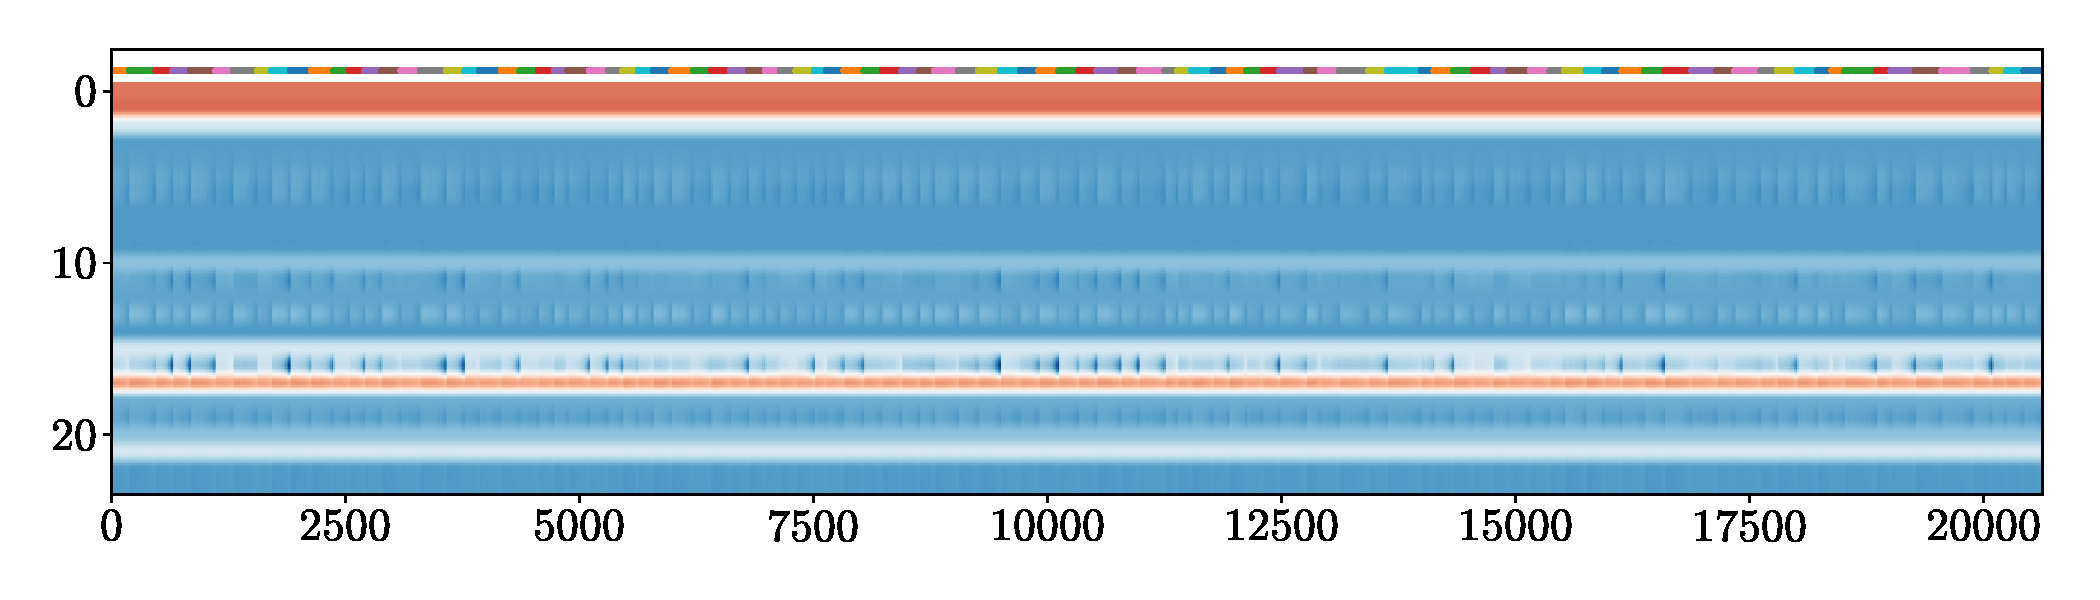
\includegraphics[width=0.95\linewidth]{./img/_rul_heatmap.pdf}
    \caption{
        \parbox[t]{0.7\linewidth}{
            Heatmap of the dataset. On the top line, each section represents an experiment.
        }
    }
\end{figure}


\subsection{Data splitting}

As the dataset is composed of experiments, standard random sampling will mix experiments and leak information. Therefore, sampling is done on the experiments in chronological order (train first).

\begin{remark}
    When splitting, the train data should be representative of the test data. Moreover, the test set should be representative of the real world.
\end{remark}


\section{Approaches}


\subsection{Regressor} \label{sec:rul_regressor}

Predict RUL with a regressor $f$ and set a threshold to trigger maintenance:
\[ f(x, \theta) \leq \varepsilon \]


\begin{description}
    \item[Linear regression]
        A linear regressor can be used as a simple baseline for further experiments.

        \begin{remark}
            For convenience, a neural network without hidden layers can be used as the regressor.
        \end{remark}

        \begin{remark}
            Training linear models with gradient descent tend to be slower to converge.
        \end{remark}

    \item[Multi-layer perceptron]
        Use a neural network to solve the regression problem.

        \begin{remark}
            A more complex model causes more training instability as it is more prone to overfitting (i.e., more variance).
        \end{remark}

        \begin{remark}
            Being more expressive, deeper models tend to converge faster.
        \end{remark}

        \begin{remark}[Self-similarity curves]
            Exponential curves (e.g., the loss decrease plot) are self-similar. By considering a portion of the full plot, the subplot will look like the whole original plot.
        \end{remark}

        \begin{remark}[Common batch size reason]
            A batch size of $32$ follows the empirical statistical rule of $30$ samples. This allows to obtain more stable gradients as irrelevant noise is reduced.
        \end{remark}

    \item[Convolutional neural network]
        Instead of feeding the network a single state, a sequence can be packed as the input using a sliding window as in \Cref{sec:ad_taxi_kde_multi}. 1D convolutions can then be used to process the input so that time proximity can be exploited.

        \begin{remark}
            Using sequence inputs might expose the model to more noise.
        \end{remark}

        \begin{remark}
            Even if the dataset is a time series, it is not always the case (as in this problem) that a sequence input is useful.
        \end{remark}
\end{description}

\begin{remark}
    The accuracy of the trained regressors are particularly poor at the beginning of the experiments due to the fact that faulty effects are noticeable only after a while. However, we are interested in predicting when a component is reaching its end-of-life. Therefore, wrong predictions when the RUL is high are acceptable.
    \begin{figure}[H]
        \centering
        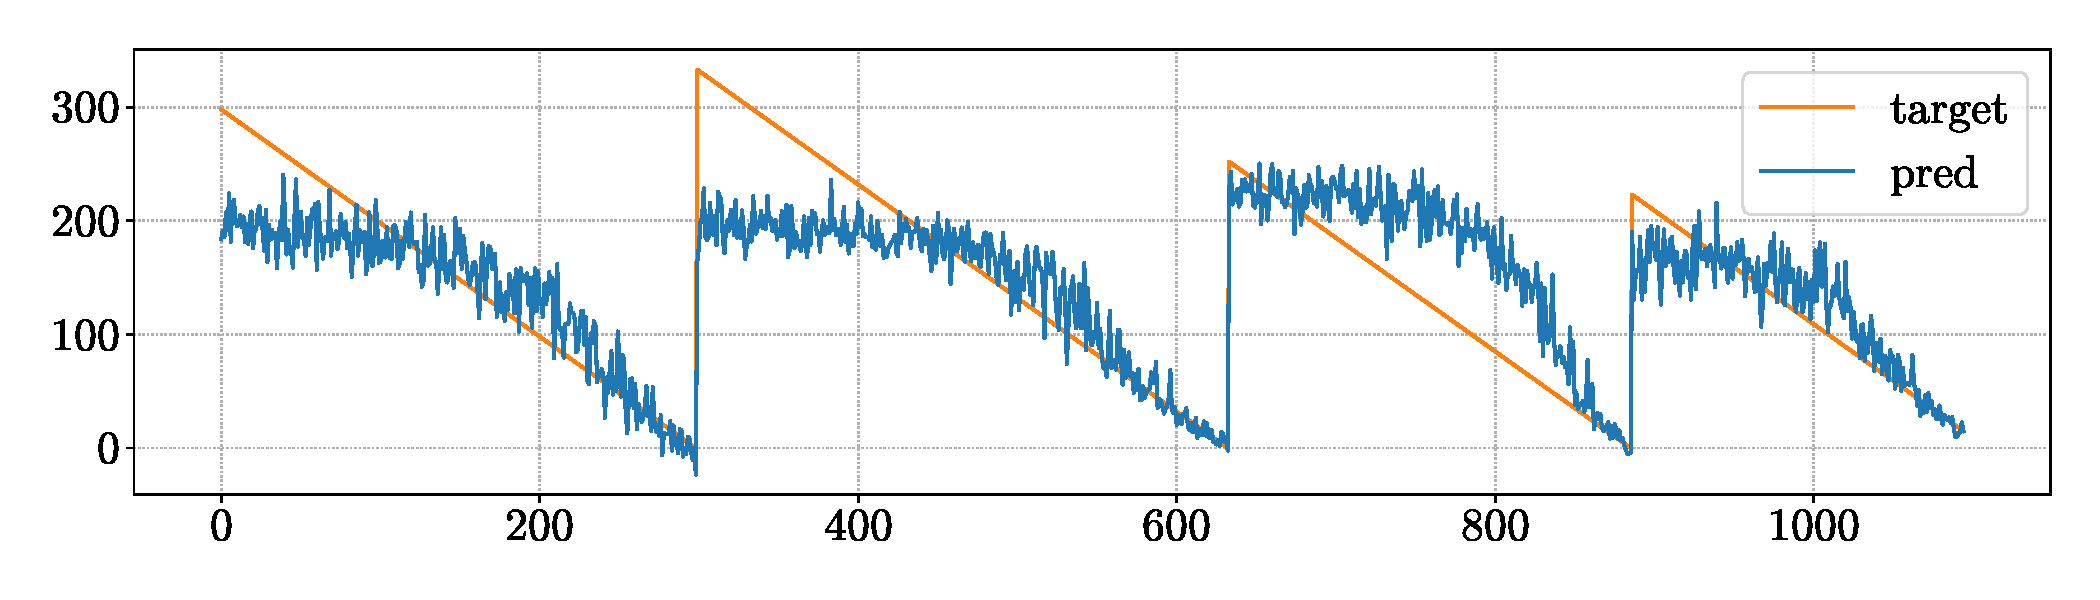
\includegraphics[width=0.7\linewidth]{./img/_rul_regression_predictions.pdf}
        \caption{Predictions on a portion of the test set}
    \end{figure}
\end{remark}

\begin{description}
    \item[Cost model] 
        Intuitively, a cost model can be defined as follows:
        \begin{itemize}
            \item The steps of the experiments are considered as the atomic value units.
            \item The cost for a failure (i.e., untriggered maintenance) is high.
            \item Triggering a maintenance too early also has a cost.
        \end{itemize}

    \item[Threshold estimation]
        To determine the threshold $\varepsilon$ that determines when to trigger a maintenance, a grid-search to minimize the cost model can be performed.

        Formally, given a set of training experiments $K$, the overall problem to solve is the following:
        \[
            \begin{split}
                \arg\min_{\varepsilon} &\sum_{k=1}^{|K|} \texttt{cost}(f(\vec{x}_k, \vec{\theta}^*), \varepsilon) \\
                &\text{ subject to } \vec{\theta}^* = \arg\min_\vec{\theta} \mathcal{L}(f(\vec{x}_k, \vec{\theta}), y_k)
            \end{split}
        \]
        Note that $\varepsilon$ do not appear in the regression problem. Therefore, this problem can be solved as two sequential subproblems (i.e., regression and then threshold optimization).
\end{description}


\subsection{Classifier}

Predict RUL with a classifier $f_\varepsilon$ (for a chosen $\varepsilon$) that determines whether a failure will occur in $\varepsilon$ steps:
\[ f_\varepsilon(x, \theta) = \begin{cases}
    1 & \text{failure in $\varepsilon$ steps} \\
    0 & \text{otherwise} \\
\end{cases} \]

\begin{remark}
    Training a classifier might be easier than a regressor.
\end{remark}

\begin{description}
    \item[Logistic regression] 
        A logistic regressor can be uses as baseline.

        \begin{remark}
            For convenience, a neural network without hidden layers can be used as the classifier.
        \end{remark}

    \item[Multi-layer perceptron]
        Use a neural network to solve the classification problem.
\end{description}

\begin{remark}
    As classifiers output a probability, they can be interpreted as the probability of not failing.
    \begin{figure}[H]
        \centering
        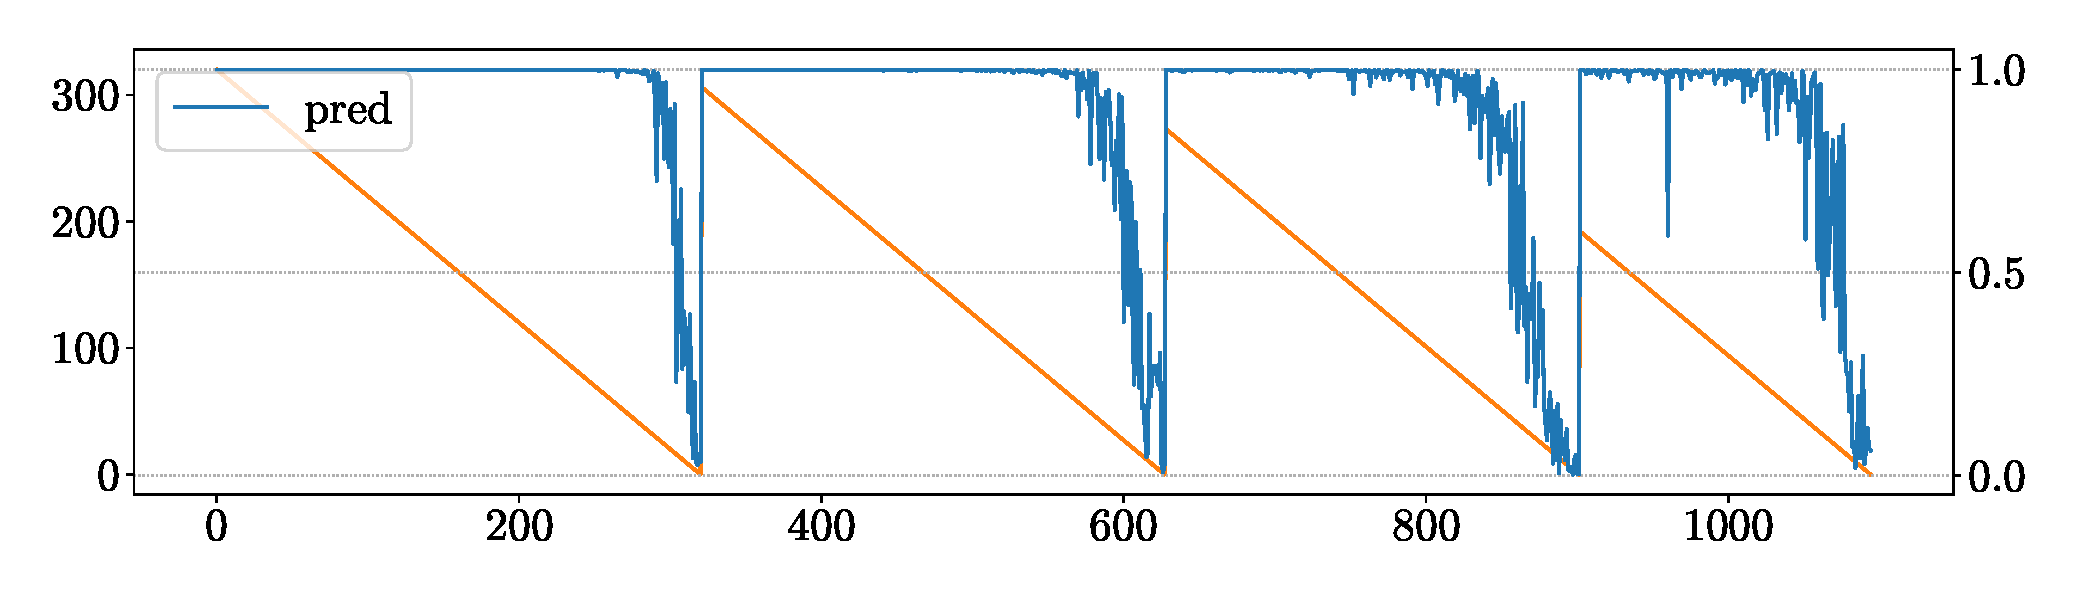
\includegraphics[width=0.7\linewidth]{./img/_rul_classification_predictions.pdf}
        \caption{Output probabilities of a classifier}
    \end{figure}
    By rounding, it is easier to visualize a threshold:
    \begin{figure}[H]
        \centering
        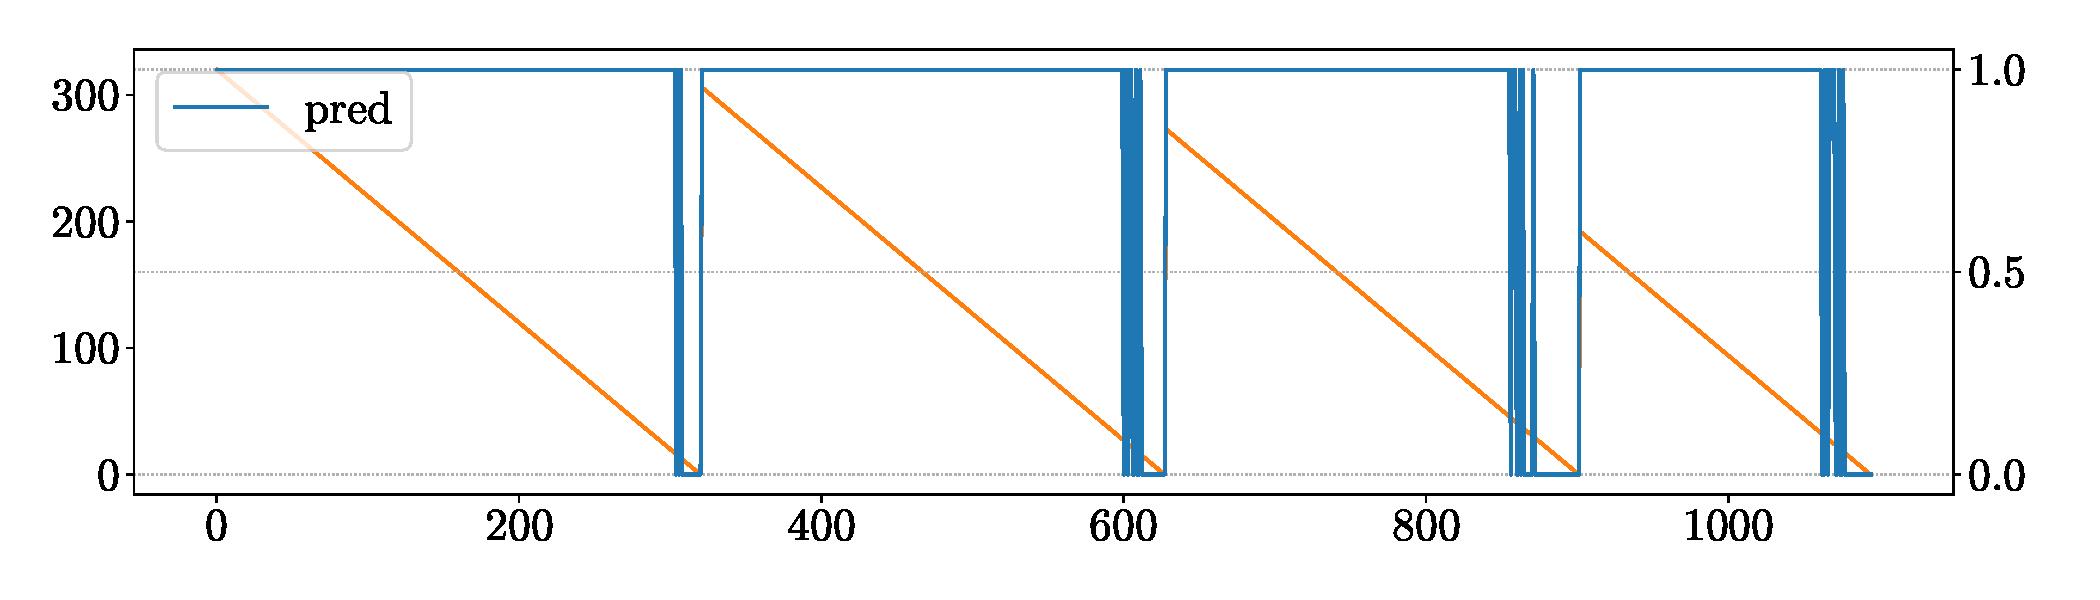
\includegraphics[width=0.7\linewidth]{./img/_rul_classification_rounding.pdf}
    \end{figure}
\end{remark}

\begin{description}
    \item[Cost model] As defined in \Cref{sec:rul_regressor}. 
    
    \item[Threshold estimation]
        \phantom{}
        \begin{remark}
            The possibility of using a user-defined threshold $\varepsilon$ allows choosing how close to a failure maintenance has to be done. However, early signs of a failure might not be evident at some thresholds so automatically optimizing it might be better.
        \end{remark}

        Formally, given a set of training experiments $K$, the overall problem to solve is the following:
        \[
            \begin{split}
                \arg\min_{\varepsilon} &\sum_{k=1}^{|K|} \texttt{cost}\left(f(\vec{x}_k, \vec{\theta}^*), \frac{1}{2}\right) \\
                &\text{ subject to } \vec{\theta}^* = \arg\min_\vec{\theta} \mathcal{L}(f(\vec{x}_k, \vec{\theta}), \mathbbm{1}_{y_k \geq \varepsilon})
            \end{split}
        \]
        Differently from regression, the threshold $\varepsilon$ appears in both the classification and threshold optimization problems, so they cannot be decomposed.

        \begin{description}
            \item[Black-box optimization] \marginnote{Black-box optimization}
                Optimization approach based on brute-force.

                For this problem, black-box optimization can be done as follows:
                \begin{enumerate}
                    \item Over the possible values of $\varepsilon$:
                        \begin{enumerate}
                            \item Determine the ground truth based on $\varepsilon$.
                            \item Train the classifier.
                            \item Compute the cost.
                        \end{enumerate}
                \end{enumerate}

                \begin{remark}
                    Black-box optimization with grid-search is very costly.
                \end{remark}

            \item[Bayesian surrogate-based optimization] \marginnote{Bayesian surrogate-based optimization}
                Method to optimize a black-box function $f$. It is assumed that $f$ is expensive to evaluate and a surrogate model (i.e., a proxy function) is instead used to optimize it.

                Formally, Bayesian optimization solves problems in the form:
                \[ \min_{x \in B} f(x) \]
                where $B$ is a box (i.e., hypercube). $f$ is optimized through a surrogate model $g$ and each time $f$ is actually used to evaluate the model, $g$ is improved.

                \begin{remark}
                    Under the correct assumptions, the result is optimal.
                \end{remark}
        \end{description}
\end{description}